\section[M2: Xtext]{M2: Xtext - textuelle Syntax}
\begin{frame}{Xtext - textuelle Syntax}
    \centering
    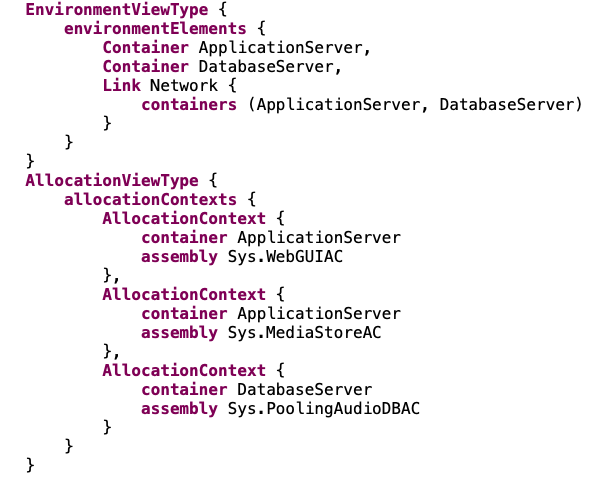
\includegraphics[height=40mm]{figures/xtext.png}
    \begin{itemize}
        \item Ergebnis: \texttt{mediastore.simplepalladio}
    \end{itemize}
\end{frame}

\begin{frame}{Probleme beim Entwurf der textuellen Syntax}
	\begin{enumerate}
		\item Import von verschiedenen Packages konnte nicht aufgelöst werden
		\begin{itemize}
            \item Lösung: Verwendung von alternativer Importschreibweise anstatt Ns URI
            \item \texttt{import "platform:/resource/SimplePalladio/..."}
        \end{itemize}
        \item Probleme mit Proxy-Ausflösung und zyklischen Abhängigkeiten
		\begin{itemize}
            \item Lösung: Grammatik als Weaving-Modell der verschiedenen Modelle in einer Datei
            \item \texttt{<datei>.simplepalladio}
        \end{itemize}
        \item OCL Constraints werden automatisch ausgewertet $\Rightarrow$ führte zu Fehlern, da OCL Constraints defekt waren
	\end{enumerate}
\end{frame}